\documentclass{../c-lecture}

\subtitle{C Programming Basics}

\begin{document}

\begin{frame}
  \titlepage{}
\end{frame}
\begin{frame}
  \frametitle{Outline}
  \tableofcontents{}
\end{frame}

\section{What is the C}

\begin{frame}
  \frametitle{The C Language}
  \begin{itemize}
    \item {\color{YellowOrange} C} is a
      {\color{YellowOrange} general-purpose} programming language
    \item {\color{LimeGreen}C} is developed by
      {\color{LimeGreen} Dennis Ritchie} at
      {\color{LimeGreen} Bell Laboratories}
    \item {\color{Orange} C} is one of the widely used languages
    \begin{itemize}
      \item Application development
      \item System programs, most operating systems are developed in C:\@ Unix, Linux
      \item Many other languages are based on it
    \end{itemize}
  \end{itemize}
\end{frame}

\begin{frame}
  \frametitle{Programming in C Language}
  \begin{itemize}
    \item C programming language
    \begin{itemize}
      \item A set of notations for representing programs
    \end{itemize}
    \item C standard libraries
    \begin{itemize}
      \item A set of developed programs (functions)
    \end{itemize}
    \item C programming environment
    \begin{itemize}
      \item A set of tools to aid program development
    \end{itemize}
  \end{itemize}
\end{frame}

\begin{frame}[fragile]
  \frametitle{The First Example}
  \begin{itemize}
    \item Write a program that prints
  \end{itemize}
  \begin{minted}[bgcolor=Black]{output}
“Hello the CE juniors :-)”
  \end{minted}
\end{frame}

\begin{frame}[fragile]
  \frametitle{The First C Program}
  \begin{minted}[bgcolor=Black]{c}
#include <stdio.h>

int main(void){
  printf("Hello the CE juniors :-) \n");
  return 0;
}
  \end{minted}
\end{frame}

\begin{frame}[fragile]
  \frametitle{General Rules}
  \begin{itemize}
    \item C is case sensitive: {\color{LimeGreen} main} is not
      {\color{Red} MaIn}

    \item A ``;'' is required after each statement
    \item Each program should have a
      {\color{Orange} main} function

    \begin{minted}[bgcolor=Black]{c}
int main(void){...
void main(void){...
main(){...
int main(int argc, char ** argv){...
    \end{minted}

    \item Program starts running from the main
    \item You should follow coding style (beautiful code)
  \end{itemize}
\end{frame}

\begin{frame}[fragile]
  \frametitle{Comments}
    \begin{minted}[bgcolor=Black]{c}
/* Our first
C program */
#include <stdio.h>

int main(void) {
  //This program prints a simple message
  printf("Hello the CE juniors :-) \n");
  return 0;
}
  \end{minted}
\end{frame}

\begin{frame}
  \frametitle{The First C Program}
  \begin{itemize}
    \item You should
    \begin{itemize}
      \item Develop the source code of program
      \item Compile
      \item Run
      \item Debug
    \end{itemize}
    \item All of them can be done in IDE
    \begin{itemize}
      \item Code::Blocks
      \item CLion
      \item VS Code
    \end{itemize}
  \end{itemize}
\end{frame}

\section{Variables}

\begin{frame}
  \frametitle{Variables}
  \begin{itemize}
    \item Solving problems
    \begin{itemize}
      \item Input data --- Algorithm --- Output data
    \end{itemize}
    \item What we need
    \begin{itemize}
      \item Implementing the algorithm
      \begin{itemize}
        \item Named {\color{Orange} Functions}
        \item We will discuss later
      \end{itemize}
      \item Storing the input/output data
      \begin{itemize}
        \item {\color{Orange} Variables}
      \end{itemize}
    \end{itemize}
  \end{itemize}
\end{frame}

\begin{frame}
  \frametitle{Variables (cont’d)}
  \begin{itemize}
    \item Data is stored in the main memory
    \item Variables
    \begin{itemize}
      \item Are the {\color{Orange} name} of locations in the main
        memory
      \begin{itemize}
        \item We use names instead of physical addresses
      \end{itemize}
      \item Specify the {\color{Green} coding} of the location
      \begin{itemize}
        \item What do the ``01''s means?
        \item What is the {\color{Cyan} type} of data?
      \end{itemize}
    \end{itemize}
  \end{itemize}
\end{frame}

\begin{frame}
  \frametitle{Variables (cont’d)}
  \begin{itemize}
    \item Variables in the C
    \begin{itemize}
      \item <Qualifier> <Type> <Identifier>
    \end{itemize}
    \item {\color{Orange} <Qualifier>}
    \begin{itemize}
      \item Is optional
      \item We will discuss later
    \end{itemize}
    \item {\color{Green}<Type>}
    \begin{itemize}
      \item Specifies the coding
    \end{itemize}
    \item {\color{Cyan}<Identifier>}
    \begin{itemize}
      \item Is the name
    \end{itemize}
  \end{itemize}
\end{frame}

\begin{frame}
  \frametitle{Types: Integers}
  \begin{itemize}
    \item Integer numbers
    \begin{itemize}
      \item Different types, different sizes, different ranges
    \end{itemize}
  \end{itemize}
\end{frame}

\begin{frame}
  \frametitle{Types: Integers}
  \begin{table}
  \begin{tabular}{cccc}
    \toprule

    Type &
    Size &
    Unsigned &
    Signed \\

    \midrule

    short &
    16 bits &
    $0 \tilde 2^{16} - 1$ &
    $-2^{15} \tilde 2^{15} - 1$ \\

    \midrule

    int &
    32 bits &
    $0 \tilde 2^{32} - 1$ &
    $-2^{31} \tilde 2^{31} - 1$ \\

    \midrule

    long --- long int &
    32/64 bits &
    $0 \tilde 2^{32/64} - 1$ &
    $-2^{31/63} \tilde 2^{31/63} - 1$ \\

    \midrule

    long long --- long long int &
    64 bits &
    $0 \tilde 2^{64} - 1$ &
    $-2^{63} \tilde 2^{63} - 1$ \\

    \bottomrule
  \end{tabular}
  \end{table}
\end{frame}

\begin{frame}
  \frametitle{Types: Float \& Double}
  \begin{itemize}
    \item Floating point number
  \end{itemize}
  \begin{table}
  \begin{tabular}{cc}
    \toprule

    float &
    32 bits \\

    \midrule

    double &
    64 bits \\

    \midrule

    long double &
    96 bits \\

    \bottomrule
  \end{tabular}
  \end{table}
  \begin{itemize}
    \item Limited precision
    \begin{itemize}
      \item float: 8 digits precision
      \item double: 16 digits precision
    \end{itemize}
  \end{itemize}
\end{frame}

\begin{frame}
  \frametitle{Overflow \& Underflow}
  \begin{itemize}
    \item All types have limited number of bits
    \begin{itemize}
      \item Limited range of number are supported
      \item Limited precision
    \end{itemize}
    \item Overflow
    \begin{itemize}
      \item Assign a very big number to a variable that is larger than the limit of
        the variable
    \end{itemize}
    \item Underflow
    \begin{itemize}
      \item Assign a very small number to a variable that is smaller than the limit
        of the variable
    \end{itemize}
  \end{itemize}
\end{frame}

\begin{frame}
  \frametitle{Types: Char}
  \begin{itemize}
    \item Character
    \begin{itemize}
      \item Type: char
    \end{itemize}
    \item Single letters of the alphabet, punctuation symbols
    \item Should be single quotation
  \end{itemize}
\end{frame}

\begin{frame}
  \frametitle{Variables: Identifier}
  \begin{itemize}
    \item
      The name of variables: {\color{Orange} identifier}
    \item
      Identifier is string ({\color{Green} single word})
    \begin{itemize}
      \item Alphabet
      \item Numbers
      \item _
    \end{itemize}
    \item But
    \begin{itemize}
      \item Can {\color{Cyan} not} start with digits
      \item
        Can {\color{Cyan} not} be the key-words (reserved
        words)
      \item Can {\color{Cyan} not} be duplicated
      \item
        Should {\color{Cyan} not} be library function names:
        \mint{c}|printf|
    \end{itemize}
  \end{itemize}
\end{frame}

\begin{frame}
  \frametitle{Variables: Identifier}
  \begin{itemize}
    \item Use readable identifiers
    \begin{itemize}
      \item Do not use memorystartaddress
      \item Use memory_start_address
      \item Do not use xyz, abc, z, x, t
      \item Use counter, sum, average, result, parameter, \ldots
      \item Do not be lazy
      \item Use meaningful names
    \end{itemize}
  \end{itemize}
\end{frame}

\begin{frame}
  \frametitle{Variables: Identifier}
  \begin{itemize}
    \item Valid identifiers
    student --- grade --- sum --- all_students --- average_grade_1
    \item Invalid identifiers
    if --- 32_test --- wrong* --- \$sds\$
  \end{itemize}
\end{frame}

\begin{frame}[fragile]
  \frametitle{Variables: Declaration}
  \begin{itemize}
    \item
      Reserve memory for variable:
      {\color{Orange} declaration}
    \begin{itemize}
      \item <type> <identifier>;
    \end{itemize}
    \item
      A variable must be declared {\color{LimeGreen} before} use
  \end{itemize}
  \begin{minted}[bgcolor=Black]{c}
char test_char;
int sample_int;
long my_long;
double sum, average, total;
int id, counter, value;
  \end{minted}
\end{frame}

\begin{frame}
  \frametitle{Variable Type Effect (in complied Lang.)}
  \begin{itemize}
    \item \textbf{\color{Orange} Important note:} the type of variable is
      NOT stored in the main memory
    \item After compiling the program, NO type is associated to memory locations!!!
  \end{itemize}
  \begin{itemize}
    \item So, what does do the type?!
    \item
      It determines the {\color{Green} operations} that work
      with the memory location
  \end{itemize}
  \begin{itemize}
    \item
      int x, y, z; z = x + y performed by {\color{Cyan} ALU}
    \item
      float a, b, c; c = a + b performed by {\color{Cyan} FPU}
  \end{itemize}
\end{frame}

\begin{frame}
  \frametitle{Variables: Initial Values}
  \begin{itemize}
    \item What this the initial value of a variable?
    \begin{itemize}
      \item In C:\@ we do not know
      \item In C:\@ it is not 0.
    \end{itemize}
  \end{itemize}
  \begin{block}
  We need to assign a value to each variable before use it.
  \end{block}
\end{frame}

\section{Values}

\begin{frame}
  \frametitle{Constants in C}
  \begin{itemize}
    \item Values
    \begin{itemize}
      \item Integer numbers
      \item Float numbers
      \item Char
      \item Strings
    \end{itemize}
    \item Symbolic constant
    \item Constant variables
  \end{itemize}
\end{frame}

\begin{frame}
  \frametitle{Values}
  \begin{itemize}
    \item Variables
    \item Declaration specifies the type and name (identifier) of variable
    \item
      Assigning value to the variable:
      {\color{Orange} assignment}

    \begin{itemize}
      \item <identifier> = <value>;
      \item
        Compute the <value> and save result in memory location specified
        by <identifier>

    \end{itemize}
  \end{itemize}
\end{frame}

\begin{frame}
  \frametitle{Values: Examples}
  \begin{minted}[bgcolor=Black]{c}
int i, j;
long l;
float f;
double d;
i = 10;
j = 20;
f = 20.0;
l = 218;
d = 19.9;
  \end{minted}
\end{frame}

\begin{frame}
  \frametitle{Value Types}
  \begin{itemize}
    \item Where are the values stored?!
    \begin{itemize}
      \item In main memory
      \item There is a logical section for these constant values
    \end{itemize}
    \item So, we need to specify the type of the value
    \begin{itemize}
      \item The coding of 01s of the value
    \end{itemize}
    \item The type of value is determined from the value itself
  \end{itemize}
\end{frame}

\begin{frame}
  \frametitle{Values: Integers}
  \begin{itemize}
    \item Valid integer values
    <p>10; -20; +400; 0x12A; 011; 5000L</p>
    \item Invalid integer values
    <p>10.0; -+20; -40 0; 600,000; 5000 L</p>
  \end{itemize}
\end{frame}

\begin{frame}
  \frametitle{Values: Float \& Double}
  \begin{itemize}
    \item Valid numbers:
    0.2; .5; -.67; 20.0; 60e10 (60 * 10^10); 7e-2 (7 * 10^-2)
    \item Invalid numbers:
    0. 2; 20. 0; 20 .0; 7 e; 6e; e12
  \end{itemize}
\end{frame}

\begin{frame}
  \frametitle{Values: Chars}
  \begin{itemize}
    \item Char values
    \begin{itemize}
      \item Should be enclosed in single quotation
    \end{itemize}
    \item Each character has a code: ASCII code
    \item Character vs. Integer
  \end{itemize}
\end{frame}

\begin{frame}
  \frametitle{Effect of Value Types}
  \begin{itemize}
    \item The type of values have the same effect of the type of variables
    \item It determines the “operations” that work on the values
  \end{itemize}
\end{frame}

\begin{frame}
  \frametitle{Basic Input Output}
  \begin{itemize}
    \item To read something: <span class="green-select">scanf</span>
    \item Integer: \mint{c}|scanf("%d", &int_variable);|
    \item Float: \mint{c}|scanf("%f", &float_variable);|
    \item Double: \mint{c}|scanf("%lf", &double_variable);|
  \end{itemize}
\end{frame}

\begin{frame}
  \frametitle{Basic Input Output}
  \begin{itemize}
    \item To print something: <span class="orange-select">printf</span>
    \item Integer: \mint{c}|printf("%d", int_variable);|
    \item Float: \mint{c}|printf("%f", float_variable);|
    \item Message: \mint{c}|printf("message");|
  \end{itemize}
\end{frame}

\section{Casting}

\begin{frame}
  \frametitle{Casting}
  \begin{itemize}
    \item What is the casting?
    \begin{itemize}
      \item
        When the type of variable and value
        {\color{Cyan} are not the same}
      \item Example: Assigning double value to integer variable
    \end{itemize}
    \item It is not a syntax error in C (only warning)
    \begin{itemize}
      \item But can cause {\color{Orange} runtime errors}
    \end{itemize}
    \item It is useful (in special situations)
    \begin{itemize}
      \item But we should be very very careful
    \end{itemize}
  \end{itemize}
\end{frame}

\begin{frame}[fragile]
  \frametitle{Implicit casting}
  \begin{itemize}
    \item Implicit
    \begin{itemize}
      \item We don’t say it
      \item But we do it
    \end{itemize}
  \end{itemize}
  \begin{minted}[bgcolor=Black]{c}
char f2 = 50e6; /* cast from double to char */
int i = 98.01; /* cast from double to int */
  \end{minted}
\end{frame}

\begin{frame}[fragile]
  \frametitle{Explicit casting}
  \begin{itemize}
    \item Explicit
    \begin{itemize}
      \item We say it
      \item And we do it
    \end{itemize}
  \end{itemize}
  \begin{minted}[bgcolor=Gray]{c}
int i = (int) 98.1; /* cast from double to int */
char c = (char) 90; /* cast from int to char */
  \end{minted}
\end{frame}

\begin{frame}[fragile]
  \frametitle{Casting effects}
  \begin{itemize}
    \item Casting from small types to large types
    \begin{itemize}
      \item There is not any problem
      \item No loss of data
    \end{itemize}
  \end{itemize}
  \begin{minted}[bgcolor=Gray]{c}
int i;
short s;
float f;
double d;
s = 'A'; // s = 65
i = 'B'; // i = 66
f = 4566; // f = 4566.0
d = 5666; // d = 5666.0
  \end{minted}
\end{frame}

\begin{frame}[fragile]
  \frametitle{Casting effects (cont’d)}
  \begin{itemize}
    \item Casting from large types to small types
    \begin{itemize}
      \item Data loss is possible
      \item Depends on the values
    \end{itemize}
  \end{itemize}
  \begin{minted}[bgcolor=Gray]{c}
float f = 65536; // 65536.0
double d = 65536; // 65536.0
short s = 720; // 720
char c = (char) 65536; // c = 0
short s = (short) 65536; // s = 0
int i = 1.22; // i = 1
int j = 1e23; // j = ???
  \end{minted}
\end{frame}

\section{Constants \& Definition}

\begin{frame}[fragile]
  \frametitle{Constant Variables}
  \begin{itemize}
    \item Constants
    \begin{itemize}
      \item Do not want to change the value
      \item Example: pi = 3.14
    \end{itemize}
    \item We can only initialize a constant variable
    \begin{itemize}
      \item We MUST initialize the constant variables (why?!)
    \end{itemize}
    \item <span class="green-select">const</span> is a qualifier
  \end{itemize}
  \begin{minted}[bgcolor=Gray]{c}
const int STUDENTS = 38;
const long int MAX_GRADE = 20;
int i;
i = MAX_GRADE;
STUDENT = 39; //ERROR
  \end{minted}
\end{frame}

\begin{frame}[fragile]
  \frametitle{Definitions}
  \begin{itemize}
    \item Another tool to define constants
    \begin{itemize}
      \item Definition is not variable
      \begin{itemize}
        \item We define definition, don’t declare them
      \end{itemize}
      \item Pre-processor replaces them by their values before compiling
    \end{itemize}
  \end{itemize}
  \begin{minted}[bgcolor=Gray]{c}
#define STUDENTS 38
int main(void) {
  int i;
  i = STUDENTS;
  STUDENTS = 90; //ERROR! What compiler sees: 38 = 90
}
  \end{minted}
\end{frame}

\begin{frame}
  \frametitle{Summary}
  \begin{itemize}
    \item Simple programs in C
    \item Two basics
    \begin{itemize}
      \item Variables
      \item Values
    \end{itemize}
    \item Casting
    \begin{itemize}
      \item The type mismatch
    \end{itemize}
  \item Constant variables \& definitions
  \end{itemize}
\end{frame}

\begin{frame}
  \frametitle{Legends}
  \begin{figure}
    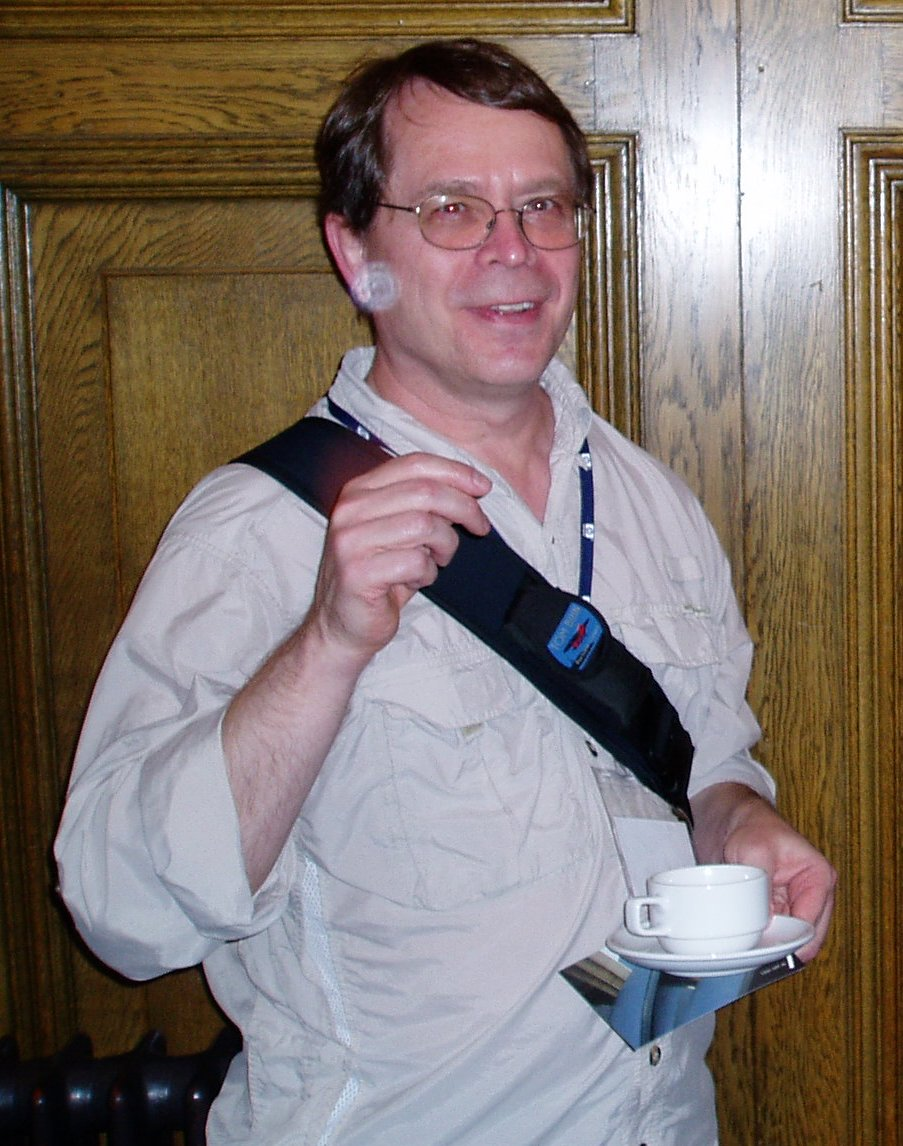
\includegraphics[height=.75\textheight]{./img/van.jpg}
  \end{figure}
  \pause%
  \centering
  \color{Violet} Van Jacobson
\end{frame}

\end{document}
